%%%%%%%%%%%%%%%%%%%%%%%%%%%%%%%%%%%%%%%%%
% Beamer Presentation
% LaTeX Template
% Version 1.0 (10/11/12)
%
% This template has been downloaded from:
% http://www.LaTeXTemplates.com
%
% License:
% CC BY-NC-SA 3.0 (http://creativecommons.org/licenses/by-nc-sa/3.0/)
%
%%%%%%%%%%%%%%%%%%%%%%%%%%%%%%%%%%%%%%%%%

%----------------------------------------------------------------------------------------
%	PACKAGES AND THEMES
%----------------------------------------------------------------------------------------

\documentclass{beamer}

\mode<presentation> {

% The Beamer class comes with a number of default slide themes
% which change the colors and layouts of slides. Below this is a list
% of all the themes, uncomment each in turn to see what they look like.

%\usetheme{default}
%\usetheme{AnnArbor}
%\usetheme{Antibes}
%\usetheme{Bergen}
%\usetheme{Berkeley}
%\usetheme{Berlin}
%\usetheme{Boadilla}
%\usetheme{CambridgeUS}
%\usetheme{Copenhagen}
%\usetheme{Darmstadt}
%\usetheme{Dresden}
%\usetheme{Frankfurt}
%\usetheme{Goettingen}
%\usetheme{Hannover}
%\usetheme{Ilmenau}
%\usetheme{JuanLesPins}
%\usetheme{Luebeck}
\usetheme{Madrid}
%\usetheme{Malmoe}
%\usetheme{Marburg}
%\usetheme{Montpellier}
%\usetheme{PaloAlto}
%\usetheme{Pittsburgh}
%\usetheme{Rochester}
%\usetheme{Singapore}
%\usetheme{Szeged}
%\usetheme{Warsaw}

% As well as themes, the Beamer class has a number of color themes
% for any slide theme. Uncomment each of these in turn to see how it
% changes the colors of your current slide theme.

%\usecolortheme{albatross}
%\usecolortheme{beaver}
%\usecolortheme{beetle}
%\usecolortheme{crane}
%\usecolortheme{dolphin}
%\usecolortheme{dove}
%\usecolortheme{fly}
%\usecolortheme{lily}
%\usecolortheme{orchid}
%\usecolortheme{rose}
%\usecolortheme{seagull}
%\usecolortheme{seahorse}
\usecolortheme{whale}
%\usecolortheme{wolverine}

%\setbeamertemplate{footline} % To remove the footer line in all slides uncomment this line
%\setbeamertemplate{footline}[page number] % To replace the footer line in all slides with a simple slide count uncomment this line

%\setbeamertemplate{navigation symbols}{} % To remove the navigation symbols from the bottom of all slides uncomment this line
}

\usepackage{graphicx} % Allows including images
\usepackage{booktabs} % Allows the use of \toprule, \midrule and \bottomrule in tables
\usepackage{mathtools}
\usepackage{textgreek}
\usepackage{MnSymbol,wasysym}
\usepackage{ragged2e}
\usepackage{csvsimple}
\usepackage{color}
\usepackage{subfig}
\justifying
\newcommand{\jwidth}{\righthyphenmin=20 \justifying}
%----------------------------------------------------------------------------------------
%	TITLE PAGE
%----------------------------------------------------------------------------------------

\title[Bayesian Model Selection]{Efficient mode jumping MCMC for Bayesian variable selection in GLMM} % The short title appears at the bottom of every slide, the full title is only on the title page
%\author{Aliaksandr Hubin} % Your name
\author[Aliaksandr Hubin]{Hubin A.A.,Storvik G.O.}
\institute[University of Oslo] % Your institution as it will appear on the bottom of every slide, may be shorthand to save space	
{
Department of Mathematics, University of Oslo \\\medskip \textit{aliaksah@math.uio.no}, \textit{geirs@math.uio.no}\\\includegraphics[height=2cm,width=7cm]{1-2-logo-universitetet-i-oslo.jpg}\\ % Your institution for the title page
UiO, Department of Astrophysics, Oslo
}
\date{30.05.2016} % Date, can be changed to a custom date

\begin{document}

\begin{frame}
\titlepage % Print the title page as the first slide
\end{frame}

%\begin{frame}
%\frametitle{Overview} % Table of contents slide, comment this block out to remove it

%\tableofcontents % Throughout your presentation, if you choose to use \section{} and \subsection{} commands, these will automatically be printed on this slide as an overview of your presentation
%\end{frame}

%----------------------------------------------------------------------------------------
%	PRESENTATION SLIDES
%----------------------------------------------------------------------------------------

%------------------------------------------------
\section{Introduction}

\begin{frame}
\frametitle{Introduction. Issues}

\begin{itemize}
\item GLMM are addressed for inference and prediction in a wide range of different applications providing a powerful scientific tool for the researchers and analysts from different fields
\item More and more sources of data are becoming available introducing a variety of hypothetical explanatory variables for these models to be considered
\item Selection of an optimal combination of these variables is crucial. Posterior model probabilities is one of the relevant measures to estimate quality of the models
\item The number of models to select from is exponential in the number of candidate variables
\item The search space in this context has numerous local extrema (potentially sparsely located)
\item Hence efficient search algorithms have to be adopted for evaluating the posterior distribution within a reasonable amount of time
\end{itemize}

\end{frame}

\section{The model} 


\begin{frame}

\frametitle{Bayesian Generalized Linear Mixed Model}

\begin{eqnarray} \label{themodeleq}
  &Y_t|\mu_t \sim  \text{f}(y|\mu_t), t \in \{1,...,T\}\\
  &\mu_t = g^{-1}\left(\eta_t\right) \\
  & \eta_t = \gamma_0\beta_0 + \sum_{i=1}^{p} \gamma_i\beta_{i}X_{ti} + \delta_t\\
 &\boldsymbol{\delta} = (\delta_1,...,\delta_T) \sim N_T\left(\boldsymbol{0},\boldsymbol{\Sigma}_b\right).
\end{eqnarray}

\begin{itemize}
\item  $\beta_i \in \mathbb{R}, i \in \{0,...,p\}$ are regression coefficients
\item $\boldsymbol{\Sigma}_b = \boldsymbol{\Sigma}_b\left(\boldsymbol{\psi}\right) \in \mathbb{R}^T\times\mathbb{R}^T$ is the covariance of the random effect $\delta_t$ 
\item $g(\cdot)$ is a proper link function
\item $\gamma_i\in\{0,1\}, i \in \{0,...,p\}$ are latent indicators  defining if covariate $X_{ti}$ is  included into the model ($\gamma_i = 1$) or not ($\gamma_i = 0$)
\end{itemize}


\end{frame}


\begin{frame}
\begin{center}
\textbf{We use a fully Bayesian approach, hence specify priors}
\end{center}
\begin{eqnarray}
&\gamma_i \sim Binom(1,q)\label{glmgammaprior}\\
&q \sim Beta(\alpha_q,\beta_q)\label{glmgammahyperprior}
\\	
&\boldsymbol\beta|\boldsymbol\gamma \sim N_{\sum_{i=1}^p{\gamma_i}}(\boldsymbol\mu_\beta,\boldsymbol\Sigma_{\beta})\label{glmbetarprior}\\
&\boldsymbol{\psi}\sim\varphi(\boldsymbol{\psi}),\label{latentprior}
\end{eqnarray}

\begin{itemize}
\item $q$ is the prior probability of including a covariate into the model
\item $\alpha_q,\beta_q$ are hyper parameters for the prior on $q$
\item $\boldsymbol\mu_\beta,\boldsymbol\Sigma_{\beta}$ are hyper parameters for the prior on $\boldsymbol\beta|\boldsymbol\gamma$
\item $\psi$ are the hyper parameters of the random effect
\end{itemize}
\end{frame}


\section{Inference} 

\begin{frame}

\frametitle{Inference on the model}

\begin{center}
\textbf{ Let:}
 \end{center} 
 
 $\theta = \{\vec{\beta},\rho,\sigma^2_{\epsilon}\}$ define parameters of the model and $\boldsymbol{\gamma}:\vec{\gamma} $ define a model itself, i.e. which covariates are addressed.
 
\begin{center}
\textit{\emph{\textbf{Then:}}}
\end{center}
\begin{itemize}
\item \jwidth $\theta|\boldsymbol{\gamma}$ define parameters conditioned on fixed models 
\item \jwidth $\exists  2^{p+1}$ different models
\end{itemize}
\begin{center}
\textit{\emph{\textbf{Goals:}}}
\end{center}
\begin{itemize}
\item \jwidth $p(\boldsymbol{\gamma},\theta|\mathbb{D})$ posterior distribution of parameters and models
\item \jwidth $p(\boldsymbol{\gamma}|\mathbb{D})$ marginal posterior distribution of the models
\item \jwidth Set of estimated models performing well in terms of some model selection criteria (MAP, WAIC, DIC, MLIK)
\end{itemize}
\end{frame}

\begin{frame}
\frametitle{Procedure}

\begin{itemize}
\item \jwidth \textbf{Note that} $p(\boldsymbol{\gamma},\theta|\mathbb{D}) = p({\theta}|\boldsymbol{\gamma},\mathbb{D})p(\boldsymbol{\gamma}|\mathbb{D})$
\item \jwidth $p(\theta|\boldsymbol{\gamma},\mathbb{D})$  and $\log p(\mathbb{D}|\boldsymbol{\gamma})$ can be efficiently obtained by INLA
\item \jwidth  \textbf{Note that} $p(\boldsymbol{\gamma}|\mathbb{D}) =  \frac{e^{\log p(\mathbb{D}|\boldsymbol{\gamma})+\log p(\boldsymbol{\gamma})}}{\sum_{\boldsymbol{\gamma}'\in\Omega_{\boldsymbol{\gamma}}}e^{\log p(\mathbb{D}|\boldsymbol{\gamma}')+\log p(\boldsymbol{\gamma}')}}$ 
\item \jwidth   $\widehat{p}(\boldsymbol{\gamma}|\mathbb{D}) =  \frac{e^{\log p(\mathbb{D}|\boldsymbol{\gamma})+\log p(\boldsymbol{\gamma})}}{\sum_{\boldsymbol{\gamma}'\in \mathbb{V}}e^{\log p(\mathbb{D}|\boldsymbol{\gamma}')+\log p(\boldsymbol{\gamma}')}}$ \item \jwidth  $\mathbb{V}$ is the subspace of $\Omega_{\boldsymbol{\gamma}}$ to be efficiently explored
\item \jwidth Note that for $p(\boldsymbol{\gamma})=p(\boldsymbol{\gamma}') \forall \boldsymbol{\gamma}, \boldsymbol{\gamma}' \in \Omega_{\boldsymbol{\gamma}}$:  
\item \jwidth $p(\boldsymbol{\gamma}|\mathbb{D}) 	\gg p(\boldsymbol{\gamma}'|\mathbb{D})$ if $\log p(\mathbb{D}|\boldsymbol{\gamma})>\log p(\mathbb{D}|\boldsymbol{\gamma}')$  often $\Longrightarrow$
 \item \jwidth\textbf{Near modal values in terms of log MLIK are particularly important} for construction of reasonable $ \mathbb{V} \subset  \Omega_{\boldsymbol{\gamma}}$, \textbf{missing} them \textbf{can dramatically influence} posterior in the original space $\Omega_{\boldsymbol{\gamma}}$
\end{itemize}
\end{frame}

\begin{frame}
\textbf{Main challenges are multimodality in $\Omega_{\boldsymbol{\gamma}}$ and its size.}
\frametitle{Possible ways to explore $\mathbb{V} \subset \Omega_{\boldsymbol{\gamma}}$}
\begin{itemize}
\item \jwidth Full enumeration of $\Omega_{\boldsymbol{\gamma}}$ - infeasible for large dimensions
\item \jwidth Random walk in $\Omega_{\boldsymbol{\gamma}}$ including simple MCMC - does not take advantage of the structure of $\Omega_{\boldsymbol{\gamma}}\Longrightarrow$ too slow 
\item \jwidth Greedy optimization with numerous initial points - end up in local optima
\item \jwidth Random walk with mode jumping proposals seems to be a good idea
\end{itemize}
\begin{figure}
\includegraphics[width=0.8\linewidth]{images/searchspace.jpg}
\end{figure}


\end{frame}

\begin{frame}

\frametitle{MCMC with locally optimized proposals}
\textbf{Tjelmeland and  Hegstad} \color{blue}[6] \color{black}    suggested continuous mode jumping proposals, \textbf{Storvik} \color{blue}[5] \color{black} considers a more general setup, \textbf{we} \textbf{suggest mode jumping proposals} in the \textbf{discrete parameter} spaces.
\begin{figure}
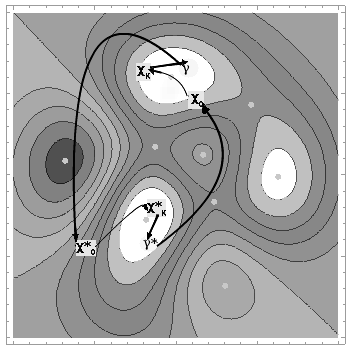
\includegraphics[width=0.45\linewidth]{images/locgreedybw1.png}
\caption{Locally optimized with randomization proposals}
\end{figure}
\end{frame}


\begin{frame}

\frametitle{Application of MCMC with mode jumping proposals}
We have shown that the detailed balance equation is satisfied for the following acceptance probabilities:

\begin{equation}
r_m(\boldsymbol{\gamma}_j,\boldsymbol{\gamma}_k) = \min\left\{1,\frac{p(\mathbb{D}|\boldsymbol{\gamma}_k)p(\boldsymbol{\gamma}_k)\mathsf{q_s}(\boldsymbol{\gamma}_j|\boldsymbol{\gamma}_{j_{K-1}})}{p(\mathbb{D}|\boldsymbol{\gamma}_j)p(\boldsymbol{\gamma}_j)\mathsf{q_s}(\boldsymbol{\gamma}_k|\boldsymbol{\gamma}_{k_{K-1}})}\right\}.\label{locmcmc3}
\end{equation}

\begin{itemize}
\item $\mathsf{q_s}(.|.)$ is the kernel of randomization at the end.
\end{itemize}

Hence we also obtain alternative MCMC estimators of posterior marginal probabilities
\begin{equation}\tilde{p}(\boldsymbol{\gamma}|\mathbb{D}) =  \frac{\sum_{i=1}^{W}{\mathbb{I}({\boldsymbol{\gamma}}_{i} = {\boldsymbol{\gamma}})}}{W} \xrightarrow[W\rightarrow\infty]{d} p(\boldsymbol{\gamma}|\mathbb{D}).
\end{equation}
\begin{itemize}
\item $W$ is the number of MCMC iterations (after burn-in)
\end{itemize}

\end{frame}

\begin{frame}
\frametitle{How it looks like in reality}
\begin{figure}
Modes are important: the standard MCMC procedure (right) misses two in this example. Visualization is challenging
\includegraphics[width=0.5\linewidth]{plots/6plot10.jpg}
\includegraphics[width=0.5\linewidth]{plots/13plot10.jpg}
\caption{MDS plots with posterior modes of all found solutions for the approaches}
\end{figure}

\end{frame}



\begin{frame}

\frametitle{Application to cosmological simulations. Cosmological hydro-simulation data (\url{http://yt-project.org/data/}).}
Observations (Bernoulli classifiers):
\begin{itemize}
\item Galaxy is quenched (or not)
\item Star hosts planet (or not)
\end{itemize}
Variables:
\begin{itemize}
\item Dark matter mass
\item Gas mass
\item Stellar mass
\item Star formation rate
\item Metallicity
\item Gas molecular fraction
\item Gas fraction
\item Stellar fraction
\item Stellar to gas mass ratio
\item Other covariates, their interactions, polynomes and etc.
\end{itemize}

\end{frame}

\begin{frame}

\frametitle{Application to NEO classification. NASA Space Challenge (\url{https://github.com/SpaceApps2016/Resources}).}
Observations (Bernoulli classifiers):
\begin{itemize}
\item Asteroid is a NEO (PHA) object or not (Phocaea)
\end{itemize}
Variables:
\begin{itemize}
\item Rotation period
\item Magnitude slope             
\item Mean anomaly
\item Inclination                    
\item Argument of perihelion          
\item Longitude of the ascending node
\item Rms residual
\item Semi major axis                
\item Eccentricity
\item Mean motion                    
\item Absolute magnitude
\item Other covariates, their interactions, polynomes and etc.
\end{itemize}

\end{frame}


\begin{frame}

\frametitle{Application to cosmological simulations or NEO objects classification}

\begin{center}
\textbf{Logistic Bayesian regression} addressed 
\end{center}


\begin{eqnarray}
&y_t = y|p_t \sim  Binom(1,p_t) \\
&p_t = \frac{e^{\gamma_0\beta_0 + \sum_{i=1}^{p} \gamma_i\beta_{i}X_{t,i}}}{1+e^{\gamma_0\beta_0 + \sum_{i=1}^{p} \gamma_i\beta_{i}X_{t,i}}}\\
&\boldsymbol\beta|\boldsymbol\gamma \sim N_{\sum_{i=1}^p{\gamma_i}}(\boldsymbol\mu_\beta,\boldsymbol\Sigma_{\beta})\\
&\gamma_i \sim Binom(1,q)\label{gammaprior}
\end{eqnarray}

\end{frame}


\begin{frame}
\frametitle{NEO objects classification. NASA space challenge}

\begin{figure}
\includegraphics[width=0.5\linewidth]{images/533px-Orbit1.png}
\includegraphics[width=0.35\linewidth]{images/apparentbrightness.jpg}
\caption{Orbital elements(left) by Lasunncty (talk), CC BY-SA 3.0 and absolute vs apparent magnitude (right) by Mrscreath( \url{http://mrscreath.blogspot.com)} }
\end{figure}

\end{frame}
\begin{frame}
\frametitle{NEO objects classification. NASA space challenge}
\begin{flushleft}
\textbf{20 covariates} addressed in the experiment (both \textit{reasonable} and \textit{heuristic}): Mean anomaly $\in [0^{\circ};360^{\circ})$\textbf{;} Argument of perihelion $\in [0^{\circ};360^{\circ})$\textbf{;}  Longitude of the ascending node $\in [0^{\circ};360^{\circ})$\textbf{;} Inclination $\in [0^{\circ};180^{\circ}]$\textbf{;} Semi major axis  $\in \bold{R^+}$\textbf{;} Eccentricity $\in \bold{R^+}$\textbf{;} Mean motion  $\in \bold{R^+}$\textbf{;} Absolute magnitude  $\in \bold{R}$ (brightness)\textbf{;} Rms residual  $\in \bold{R^+}$(brightness error)\textbf{;} Eccentricity$^2$ $\in \bold{R^+}$\textbf{;} Absolute magnitude$^2$ $\in \bold{R^+}$\textbf{;} Semi major axis$^2$ $\in \bold{R^+}$\textbf{;} Semi major axis$^3$ $\in \bold{R^+}$\textbf{;} Mean anomaly$\times$Semi major axis\textbf{;}  Mean anomaly$\times$Semi major axis$^2$ $\in \bold{R^+}$\textbf{;} Mean anomaly$\times$Semi major axis$^3$ $\in \bold{R^+}$\textbf{;} Argument of perihelion$\times$Semi major axis $\in \bold{R^+}$\textbf{;}  Argument of perihelion$\times$Semi major axis$^2$ $\in \bold{R^+}$\textbf{;} Argument of perihelion$\times$Semi major axis$^3$ $\in \bold{R^+}$\textbf{;} Longitude of the ascending node$\times$Semi major axis $\in \bold{R^+}$.
\end{flushleft}
\begin{flushleft}
\textbf{Training set} includes 32 NEO and 32 non-NEO objects, \textbf{test set} includes 20720 objects (14099 NEO,  6621 non-NEO),  \textbf{validation sets} were used as some random subsets of a 100 elements from these  20720 \textbf{objects}
\begin{flushleft}
\textbf{$\bold{2^{20}}$ models} in total, algorithm was run until ca \textbf{2500 models} and ca \textbf{10000 models} are visited.
\end{flushleft}

\end{flushleft}

\end{frame}

\begin{frame}
\frametitle{NEO objects classification. Inference}
\begin{figure}
Posterior inclusion probabilities and posterior model probabilities
\includegraphics[width=0.5\linewidth]{plots/astrorm.jpeg}
\includegraphics[width=0.5\linewidth]{plots/modpost.jpg}
\caption{Comparison of marginal inclusion probabilities of the covariates (left) and models on the whole (right)}
\end{figure}

\end{frame}


\begin{frame}
\frametitle{NEO objects classification. Bayesian classification}
Choice of $\mathbb{V}^*$ is crucial, $\mathbb{V}^*=\Omega_{\boldsymbol{\gamma}}$ - often in-feasible, $\mathbb{V}^*=\mathbb{V}$ - very precise can be too slow, $\mathbb{V}^*= \mathbb{V}\cap p(\boldsymbol{\gamma}|\mathbb{D})\geq\alpha$ - often precise, but is a way faster!!!
\begin{figure}
\includegraphics[width=0.6\linewidth]{images/ANN.png}
\caption{Bayesian Artificial Neuron Network for Classification}
 $\hat{Y}=\mathbb{I}\{\hat{\text{E}}[Y|\boldsymbol{\mathsf{D}}]\geq0.5\},  \hat{\text{E}}[Y|\boldsymbol{\mathsf{D}}]=  \sum_{\boldsymbol{\boldsymbol{\gamma}} \in  \mathbb{V}^*}{\hat{\text{E}}[y_{\gamma}|\boldsymbol{\gamma},\boldsymbol{\mathsf{D}}]\hat{p}(\boldsymbol{\gamma}|\boldsymbol{\mathsf{D}})}$
\end{figure}

\end{frame}


\begin{frame}
\frametitle{NEO objects classification. Results}
\begin{center}
Quite impressive actually... Surprisingly or not?.. Comments?..\\
\textbf{Remember: $||$training set$||=64$, $||$test set$||=20720$}
\end{center}

\tiny
\begin{table}[t]
\begin{tabular}{ 
|l|c|c|c|c|c|c|c|}
\hline
Subset&$||$Hidden$||$&Precision&FNR&FPR&Time&Time/it.\\\hline
$\mathbb{V}^1$&10090&99.95656\%&0.05670945
\%&0.01510117
\%&619.89 min&1.795 sec\\
$\mathbb{V}^2$&2512&99.80212\%&0.05670945
\%&0.49594239
\%&172.66 min&0.499 sec\\
$\mathbb{V}^3$&412&99.46429\%&0.04253813
\%&1.56110622\%&29.166 min&0.084 sec\\
$\mathbb{V}^4$&80&99.19402\%&0.02836276\%&2.40271201\%&9.9812 min&0.029 sec\\
$\mathbb{V}^5$&4&90.00483\%& 0.04962427
\%&23.7651171
\%&4.7789 min&0.014 sec\\
$\text{argmax}_{\boldsymbol{\gamma} \in \mathbb{V}^1}\{{p_{\mathbb{V}}(\boldsymbol{\gamma}|\mathbb{D})}\}$&1& 82.83301\%& 0.07087675
\%&34.8839473
\%&4.5222 min&0.013 sec\\
Wake up NEO &?&93.86271\%&1.00000000\%&17.0000000\%&-&-\\\hline

\end{tabular}
\\[1pt]
\caption{Comparison of performance (Precision, FDR, FNR, Time) of different models}
\end{table}

N/B: the best model includes eccentricity$^2$, eccentricity, absolute magnitude$^2$, absolute magnitude 
\end{frame}

\begin{frame}
\frametitle{Multicore and shared memory issues}

\begin{figure}
\includegraphics[width=0.43\linewidth]{multicpu.png}
\caption{Multiprocessing architecture}
\end{figure}
\end{frame}

\begin{frame}
\frametitle{The protein activity data. $2^{88}$ models. Multiple modes}
\begin{figure}
Comparison to other algorithms: BAS, RS (simper MCMC) on $2^{20}$ unique models visited for MJMCMC and BAS and $88\times 2^{20}$ iterations of RS.
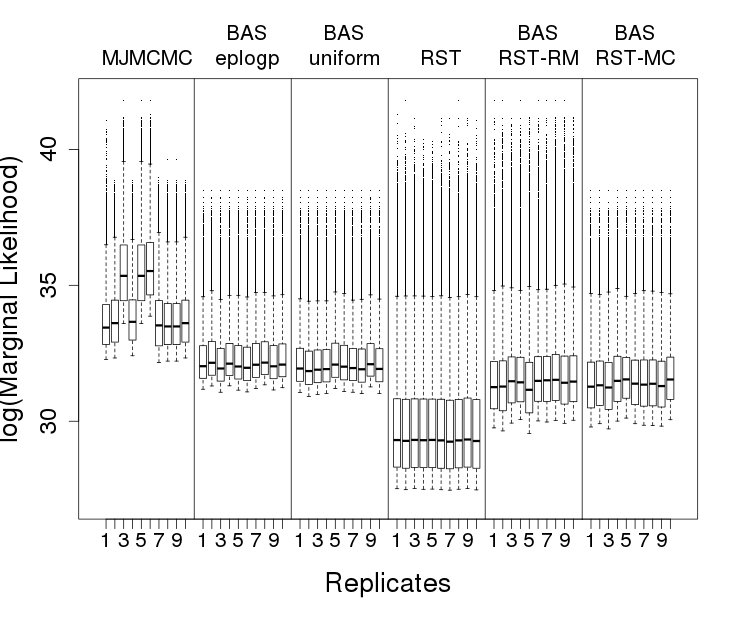
\includegraphics[width=0.5\linewidth]{images/mliks.jpeg}
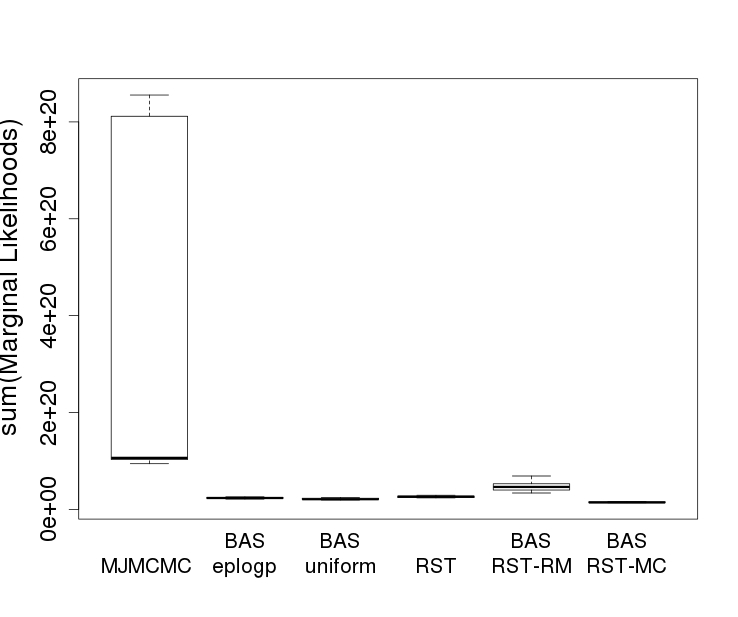
\includegraphics[width=0.5\linewidth]{images/massesbig.jpeg}
\caption{100000 best mliks found (left) and posterior masses captured ({right}). Bayesian linear regression with a g-prior is addressed, since no other packages (to our awareness) manage model selection in GLMM}
\end{figure}

\end{frame}

\begin{frame}
\frametitle{The protein activity data. $2^{88}$ models.  Multiple modes}
\begin{figure}
Checking convergence. Marginal inclusion probabilities
\includegraphics[width=0.5\linewidth]{images/marginrm.jpeg}
\includegraphics[width=0.5\linewidth]{images/marginmc.jpeg}
\caption{Comparison of marginal inclusion probabilities obtained by the Bayes formula and MCMC approximations from the best run of MJMCMC with $8.56\text{e}+20$ posterior mass captured}
\end{figure}

\end{frame}


\section{Conclusions}

\begin{frame}
\frametitle{Concluding remarks}

\begin{itemize}
\item \jwidth We introduced the MJMCMC approach for estimating posterior model probabilities and Bayesian model averaging and selection. 
\item \jwidth It incorporates the ideas of MCMC with possibility of large jumps combined with local optimizers to generate proposals in the discrete space of models
\item \jwidth \textit{EMJMCMC} R-package is developed and available from the GitHub repository: \url{http://aliaksah.github.io/EMJMCMC2016/}
\item \jwidth The developed package gives a user high flexibility in the choice of methods to obtain marginal likelihoods and model selection criteria within GLMM
\item \jwidth  Extensive parallel computing for both MCMC moves and local optimizers is available within the developed package
\item \jwidth Based on the obtained in the experimental part results, we can claim MJMCMC to be a rather competitive novel algorithm that both performs well in terms of the search quality and addressed a more general class of statistical models than the competing approaches
\end{itemize}

\end{frame}

\begin{frame}
\frametitle{References}
%@misc{1604.06398,
%author = {Aliaksandr Hubin and Geir Storvik},
%title = {{E}fficient mode jumping {MCMC} for {B}ayesian variable selection in {GLMM}},
%year = {2016},
%eprint = {1604.06398},
%note = {arXiv:1604.06398v1}
%}

\begin{figure}
\small
\begin{thebibliography}{\small}
\bibitem[Clyde et~al.(2010)Clyde, Ghosh, and Littman]{Clyde:Ghosh:Littman:2010}
M.~Clyde, J.~Ghosh, and M.~Littman.
\newblock Bayesian adaptive sampling for variable selection and model
  averaging.
\newblock \emph{Journal of Computational and Graphical Statistics}, 20\penalty0
  (1):\penalty0 80--101, 2011.
  
\bibitem[Hubin and Storvik(2005)]{MJMCMC2016}
A.~Hubin and G.O.~Storvik
\newblock \emph{{E}fficient mode jumping {MCMC} for {B}ayesian variable selection in {GLMM}}.
\newblock arXiv:1604.06398v1, 2016.

\bibitem[Rue et~al.(2009)Rue, Martino, and Chopin]{rue2009eINLA}
H.~Rue, S.~Martino, and N.~Chopin.
\newblock Approximate bayesian inference for latent gaussian models by using
  integrated nested laplace approximations.
\newblock \emph{Journal of the Royal Statistical Sosciety}, 71\penalty0
  (2):\penalty0 319--392, 2009.

\bibitem[Storvik(2011)]{geirs2011mhf}
G.O.~Storvik.
\newblock On the flexibility of metropolis-hastings acceptance probabilities in
  auxiliary variable proposal generation.
\newblock \emph{Scandinavian Journal of Statistics}, 38:\penalty0 342--358,
  2011.


\end{thebibliography}
\end{figure}

\end{frame}

\begin{frame}
\Huge{\centerline{The End.}}
\begin{center}

\begin{figure}
\includegraphics[width=0.8\linewidth]{images/epigenetics.jpg}
\end{figure}


Thank you.
\end{center}
\end{frame}


\end{document} 
